% ============================================================
%  Présentation Beamer — Mémoire d'épistémologie de l'informatique
%  "Que deviennent les notions de compétence et de réussite scolaire
%   dans un monde où les IAG sont en plein essor ?"
%  Ivan LEJEUNE — Master 1 Algorithmique — Université de Montpellier
% ============================================================



% -------- Thème et couleurs --------
\usetheme{Madrid}
\usecolortheme{seahorse}

% Couleurs personnalisées Université de Montpellier
\definecolor{umbleu}{RGB}{0, 62, 126}
\definecolor{umclair}{RGB}{180, 210, 240}
\definecolor{accent}{RGB}{220, 50, 50}

\setbeamercolor{frametitle}{bg=umbleu, fg=white}
\setbeamercolor{title}{fg=umbleu}
\setbeamercolor{structure}{fg=umbleu}
\setbeamercolor{block title}{bg=umbleu, fg=white}
\setbeamercolor{block body}{bg=umclair!40}
\setbeamercolor{block title alerted}{bg=accent, fg=white}
\setbeamercolor{block body alerted}{bg=accent!10}
\setbeamercolor{footline}{bg=umbleu!90, fg=white}

% -------- Packages --------
\usepackage[provide=*,french]{babel}
\usepackage[utf8]{inputenc}
\usepackage[T1]{fontenc}

\usepackage[activate=false]{microtype}
\usepackage{tikz}
\usetikzlibrary{arrows.meta, positioning, shapes.geometric}

% -------- Métadonnées --------
\title[IAG et réussite scolaire]{%
  Que deviennent les notions de compétence\\
  et de réussite scolaire dans un monde\\
  où les IAG sont en plein essor~?}
\subtitle{Mémoire d'épistémologie de l'informatique}
\author[Ivan Lejeune]{Ivan \textsc{Lejeune}}
\institute[Univ. Montpellier]{%
  Master 1 Algorithmique\\
  Université de Montpellier --- Faculté des Sciences\\[0.3em]
  \small Encadré par Bruno \textsc{Durand}}
\date{31 mai 2026}



% -------- Pied de page personnalisé --------
\setbeamertemplate{footline}{%
  \leavevmode%
  \hbox{%
    \begin{beamercolorbox}[wd=.35\paperwidth,ht=2.4ex,dp=1ex,leftskip=1em]{footline}%
      \usebeamerfont{author in head/foot}Ivan Lejeune
    \end{beamercolorbox}%
    \begin{beamercolorbox}[wd=.45\paperwidth,ht=2.4ex,dp=1ex,center]{footline}%
      \usebeamerfont{title in head/foot}\insertshorttitle
    \end{beamercolorbox}%
    \begin{beamercolorbox}[wd=.20\paperwidth,ht=2.4ex,dp=1ex,rightskip=1em,right]{footline}%
      \usebeamerfont{date in head/foot}\insertframenumber{}/\inserttotalframenumber
    \end{beamercolorbox}}%
}
\setbeamertemplate{navigation symbols}{}

% ============================================================
\begin{document}
% ============================================================

% -------- DIAPOSITIVE 1: Titre --------
\begin{frame}[plain]
  \titlepage
  
% 
\includegraphics{./images/UM1.png} %
% or with small size
\vspace{-2cm}

\includegraphics[height=1.5cm]{./images/UM1.png} %
\hfill

\includegraphics[height=1.5cm]{./images/FDS1.png} %
\end{frame}

% -------- DIAPOSITIVE 2: Plan --------
\begin{frame}{Plan de la présentation}
  \tableofcontents[hideallsubsections]
\end{frame}

% ============================================================
\section{Contexte et problématique}
% ============================================================

\begin{frame}{L'irruption des IAG dans l'espace éducatif}
  \begin{itemize}
    \item Lancement grand public de ChatGPT fin 2022
    \item Diffusion massive et rapide dans les pratiques étudiantes
    \item L'IA en éducation a une histoire longue (années 1950--1980)
          --- mais une rupture \emph{qualitative} avec les IAG
  \end{itemize}
  \vspace{0.8em}
  \begin{alertblock}{Ce qui est radicalement nouveau}
    La capacité de générer du contenu en \textbf{langage naturel}
    indiscernable d'une production humaine.
  \end{alertblock}
\end{frame}

\begin{frame}{La problématique centrale}
  \begin{block}{Question de recherche}
    \centering\large
    Si un outil peut produire en quelques secondes\\
    un travail formellement irréprochable,\\[0.4em]
    \textbf{que mesurent encore nos évaluations~?}\\
    \textbf{Que signifie encore réussir à l'école, ou être compétent~?}
  \end{block}

  \vspace{0.8em}

  \begin{itemize}
    \item Ce n'est \emph{pas} une question organisationnelle ou technique
    \item Elle touche aux \textbf{fondements épistémologiques} du système scolaire
    \item L'IAG agit comme un \textbf{révélateur}: elle met à nu des présupposés
          que l'école n'avait pas eu besoin d'expliciter
  \end{itemize}
\end{frame}

\begin{frame}{La problématique centrale}
  \begin{block}{Objectif du mémoire}
    \textbf{Décrire et analyser ces tensions} ---
    pas proposer un système éducatif alternatif.
  \end{block}
\end{frame}

% ============================================================
\section{Définitions et cadre théorique}
% ============================================================

\begin{frame}{Compétence et réussite scolaire: définitions}
  \begin{columns}[T]
    \begin{column}{0.48\textwidth}
      \begin{block}{Compétence (Perrenoud, 1999)}
        «~Capacité d'action efficace face à une famille
        de situations~» impliquant mobilisation \emph{et}
        transfert des savoirs.
      \end{block}
      \vspace{0.4em}
      \begin{block}{Ressources externes (Tardif, 2006)}
        La compétence mobilise des ressources \textbf{internes
        et externes} --- ce qui rend la question des IAG
        comme ressource \emph{délicate}.
      \end{block}
    \end{column}
    \begin{column}{0.48\textwidth}
      \begin{block}{Réussite scolaire}
        Notes, passage de classe, diplôme ---
        mais une tension fondamentale:
        mesure-t-on des compétences réelles
        ou une \emph{conformité aux codes institutionnels}~?
      \end{block}
      \vspace{0.4em}
      \begin{alertblock}{Bourdieu \& Passeron (1970)}
        La réussite récompense le \textbf{capital culturel},
        pas le mérite individuel.\\
        Les IAG \emph{radicalisent} cette déconstruction.
      \end{alertblock}
    \end{column}
  \end{columns}
\end{frame}

\begin{frame}{Cadre théorique: deux piliers}
  \begin{columns}[T]
    \begin{column}{0.48\textwidth}
      \begin{block}{Transposition didactique (Chevallard, 1985)}
        Le savoir scolaire est une version \emph{transformée}
        du savoir savant --- décontextualisé, normé.\\[0.4em]
        L'approche par compétences cherche à corriger cet
        écart, mais ce faisant, elle \textbf{expose l'évaluation
        aux outils réels} --- comme les IAG.
      \end{block}
    \end{column}
    \begin{column}{0.48\textwidth}
      \begin{block}{Légitimité scolaire (Bourdieu)}
        Les critères d'évaluation valorisent un rapport
        au savoir \emph{culturellement arbitraire}.\\[0.4em]
        Les IAG le mettent en évidence: si une machine
        satisfait ces critères, \textbf{qu'est-ce qu'ils
        mesurent vraiment~?}
      \end{block}
    \end{column}
  \end{columns}
\end{frame}

% ============================================================
\section{Les IAG face aux évaluations}
% ============================================================

\begin{frame}{Comment les IAG fragilisent l'évaluation}
  \begin{columns}[T]
    \begin{column}{0.52\textwidth}
      \textbf{L'évaluation traditionnelle supposait:}
      \begin{itemize}
        \item Un travail authentiquement individuel
        \item Un effort cognitif observable dans le rendu
        \item Une cohérence entre performance et capacités
      \end{itemize}
      \vspace{0.6em}
      \textbf{Ce que les IAG changent:}
      \begin{itemize}
        \item Texte structuré et argumenté en quelques minutes
        \item \textbf{Aucune trace} dans le rendu final
        \item Les détecteurs IA: faux positifs, faux négatifs --- insuffisants
      \end{itemize}
    \end{column}
    \begin{column}{0.44\textwidth}
      \begin{alertblock}{La distinction cruciale (Shiohira, 2021)}
        \textbf{Substitut}: l'IAG remplace le processus cognitif\\[0.3em]
        \textbf{Outil}: l'IAG amplifie et soutient ce processus\\[0.5em]
        \emph{Indiscernables à partir du seul rendu final.}
      \end{alertblock}
    \end{column}
  \end{columns}
\end{frame}


\begin{frame}{Interdiction vs intégration}
  \begin{columns}[T]
    \begin{column}{0.48\textwidth}
      \begin{block}{Position 1: Interdiction}
        \textbf{Argument}: intégrité académique ---
        déléguer c'est rompre le lien entre
        travail remis et compétences réelles.\\[0.4em]
        \textbf{Forces}: préserve la valeur
        des certifications, maintient l'effort
        formateur.\\[0.4em]
        \textbf{Limite profonde}: suppose que
        les critères actuels sont valides ---
        sans le vérifier.
      \end{block}
    \end{column}
    \begin{column}{0.48\textwidth}
      \begin{block}{Position 2: Intégration}
        \textbf{Argument}: réalisme pédagogique ---
        les IAG transforment déjà le monde
        professionnel.\\[0.4em]
        \textbf{Forces}: prépare les apprenants,
        personnalisation, démocratisation
        potentielle.\\[0.4em]
        \textbf{Limite profonde}: sans refonte
        des critères, certifie des performances
        sans compétences réelles.
      \end{block}
    \end{column}
  \end{columns}
\end{frame}

% ============================================================
\section{Deux positions institutionnelles}
% ============================================================

\begin{frame}{Interdiction vs intégration}
  \begin{alertblock}{Limite partagée}
    Les deux traitent le problème comme une \textbf{régulation de l'outil}
    sans interroger la \textbf{validité des critères d'évaluation}.
  \end{alertblock}
\end{frame}

% ============================================================
\section{Quatre tensions épistémologiques}
% ============================================================

\begin{frame}{Vue d'ensemble des quatre tensions}
  \centering
  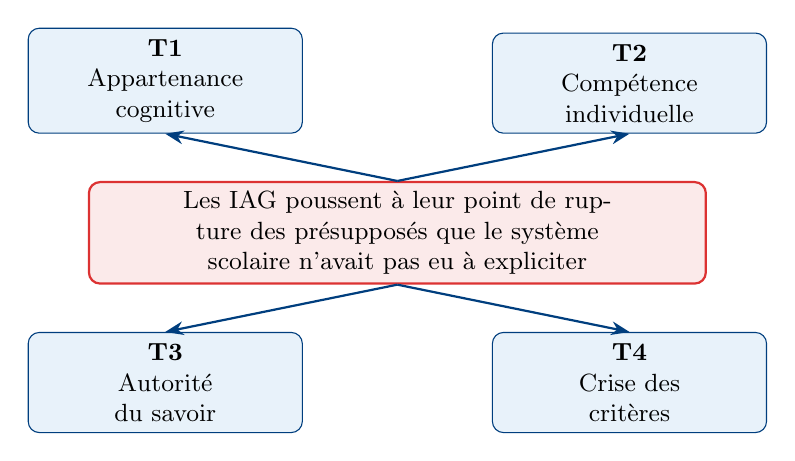
\begin{tikzpicture}[
    node distance=0.6cm and 1.2cm,
    box/.style={draw=umbleu, rounded corners, fill=umclair!30,
                text width=3.2cm, align=center, font=\small,
                minimum height=1.1cm, inner sep=4pt},
    arrow/.style={-{Stealth}, thick, umbleu}
  ]
    % Central main bubble
    \node[draw=accent, thick, rounded corners, fill=accent!10,
          text width=7.6cm, align=center, font=\small]
      (iag) {Les IAG poussent à leur point de rupture des présupposés
             que le système scolaire n'avait pas eu à expliciter};

    % Top bubbles (T1 and T2) - Further spaced out horizontally
    \node[box, above left=0.6cm and 1.2cm of iag.north] (t1) {\textbf{T1}\\Appartenance\\cognitive};
    \node[box, above right=0.6cm and 1.2cm of iag.north] (t2) {\textbf{T2}\\Compétence\\individuelle};

    % Bottom bubbles (T3 and T4) - Further spaced out horizontally
    \node[box, below left=0.6cm and 1.2cm of iag.south] (t3) {\textbf{T3}\\Autorité\\du savoir};
    \node[box, below right=0.6cm and 1.2cm of iag.south] (t4) {\textbf{T4}\\Crise des\\critères};

    % Arrows
    \draw[arrow] (iag.north) -- (t1.south);
    \draw[arrow] (iag.north) -- (t2.south);
    \draw[arrow] (iag.south) -- (t3.north);
    \draw[arrow] (iag.south) -- (t4.north);
  \end{tikzpicture}
\end{frame}

\begin{frame}{Tension 1 --- Appartenance cognitive}
  \begin{columns}[T]
    \begin{column}{0.54\textwidth}
      \textbf{La question:} à qui appartient un travail
      produit avec une IAG~?\\[0.6em]
      \begin{itemize}
        \item \textbf{Tardif (2006)}: la compétence mobilise
              des ressources \emph{externes} --- l'IAG
              pourrait être légitime comme un dictionnaire.
        \item Mais la compétence exige aussi
              l'\emph{intériorisation} et le
              \emph{transfert} à des situations nouvelles.
        \item Si la capacité dépend entièrement de
              l'outil, elle n'est pas généralisable.
      \end{itemize}
    \end{column}
    \begin{column}{0.42\textwidth}
      \begin{alertblock}{Le problème des traces}
        Calculatrice: calculs intermédiaires
        absents → usage détectable.\\[0.3em]
        IAG: \textbf{aucune marque formelle}
        dans le texte produit.\\[0.3em]
        L'évaluation présumait une cohérence
        performance / capacités: \textbf{cette
        présomption est brisée}.
      \end{alertblock}
      \vspace{-0.5em}
      \begin{block}{Réponse partielle}
        Évaluer le \textbf{processus} observable
        plutôt que le seul produit final.
      \end{block}
    \end{column}
  \end{columns}
\end{frame}

\begin{frame}{Tension 2 \& 3 --- Individu et autorité du savoir}
  \begin{columns}[T]
    \begin{column}{0.48\textwidth}
      \begin{block}{T2: Compétence individuelle}
        Le système certifie des \emph{individus} ---
        présupposé méritocratique déjà fragile
        (Bourdieu: capital culturel familial).\\[0.4em]
        Les IAG \textbf{radicalisent} cette déconstruction:
        si une machine peut satisfaire les critères,
        que mesure-t-on vraiment~?\\[0.4em]
        \emph{Réponse:} évaluer comment l'apprenant
        interagit avec les outils --- la compétence
        \textbf{dans} un écosystème outillé.
      \end{block}
    \end{column}
    \begin{column}{0.48\textwidth}
      \begin{block}{T3: Autorité épistémique}
        Traditionellement: l'enseignant détient
        et médie le savoir légitime.\\[0.4em]
        Les IAG exercent une \textbf{autorité
        épistémique concurrente} --- elles synthétisent
        directement, sans passer par l'institution.\\[0.4em]
        Le rôle enseignant se déplace:
        transmetteur → \textbf{formateur à l'évaluation
        critique des sources}.
      \end{block}
    \end{column}
  \end{columns}
\end{frame}

\begin{frame}{Tension 4 --- La crise des critères}
  \begin{block}{Le contrat didactique perverti}
    Les évaluations récompensaient la conformité formelle
    plus que la compétence réelle.
  \end{block}

  \vspace{0.5em}

  \begin{columns}[T]
    \begin{column}{0.48\textwidth}
      Une IAG pendant son entraînement optimise
      une fonction d'objectif définie par des
      évaluateurs humains, \emph{sans que cet objectif
      capture nécessairement ce qu'on cherche vraiment}.\\[0.3em]
      \(\rightarrow\) L'apprenant et l'IAG partagent
      \textbf{le même comportement d'optimisation}.
    \end{column}
    \begin{column}{0.49\textwidth}
      \begin{alertblock}{Une opportunité épistémologique}
        Si une machine satisfait nos critères,
        c'est une invitation à en formuler des
        \textbf{meilleurs}
        \begin{itemize}
          \item Réflexivité sur son apprentissage
          \item Évaluation critique d'une production IA
        \end{itemize}
      \end{alertblock}
    \end{column}
  \end{columns}
\end{frame}

% ============================================================
\section{Discussion et conclusion}
% ============================================================

\begin{frame}{Ce que les tensions impliquent}
  \begin{columns}[T]
    \begin{column}{0.48\textwidth}
      \begin{block}{L'interdiction échoue sur T1 et T4}
        Elle préserve la \emph{forme} des évaluations
        sans interroger leur \emph{validité}.\\
        Elle est en contradiction interne avec la
        définition de la compétence: exclure une
        ressource pertinente exige une justification,
        pas un décret.
      \end{block}
    \end{column}
    \begin{column}{0.48\textwidth}
      \begin{block}{L'intégration naïve échoue sur T2 et T3}
        Sans redéfinition des critères et sans
        rendre le processus observable, elle certifie
        des performances sans compétences réelles.\\
        Savoir utiliser une IAG $\neq$ avoir développé
        une pensée critique.
      \end{block}
    \end{column}
  \end{columns}
\end{frame}

\begin{frame}{Ce que les tensions impliquent}

  \begin{alertblock}{Le diagnostic d'Alexandre (2019)}
    Si l'école se définit par la \emph{restitution} de savoirs formalisés,
    les IAG la rendent effectivement obsolète.\\
    La réponse: déplacer l'accent de la \textbf{restitution}
    vers la \textbf{production} --- former des apprenants qui
    questionnent, situent et produisent des savoirs nouveaux.
  \end{alertblock}
\end{frame}

\begin{frame}{Conclusion}
  \begin{block}{Réponse à la question posée}
    Les notions de compétence et de réussite scolaire
    \textbf{ne disparaissent pas} --- elles \textbf{se complexifient}
    en révélant des tensions que le système portait déjà.
  \end{block}

  \vspace{0.5em}

  \begin{itemize}
    \item \textbf{Compétence}: ne peut plus ignorer les outils cognitifs
          externalisés --- mais ne peut pas s'y réduire.
    \item \textbf{Réussite}: redéfinir ce que l'école veut certifier.
    \item \textbf{Évaluation}: passer de «~qu'a produit l'apprenant~?~»
          à «~comment construit-il sa pensée avec ses outils~?~»
  \end{itemize}
\end{frame}


% -------- DIAPOSITIVE FINALE: Merci / Questions --------
\begin{frame}[plain]
  \vfill
  \centering
  {\Large\bfseries\color{umbleu} Merci pour votre attention}

  \vspace{1.5em}

  {\large Questions~?}

  \vspace{2em}

  
\begin{tikzpicture}
    \draw[thick, umbleu] (0,0) -- (9,0);
  \end{tikzpicture}

  \vspace{1.5em}

  \begin{columns}[c]
    \begin{column}{0.45\textwidth}
      \centering
      {\small \textbf{Ivan Lejeune}}\\
      {\footnotesize Master 1 Algorithmique}\\
      {\footnotesize Université de Montpellier}
    \end{column}
    \begin{column}{0.45\textwidth}
      \centering
      {\small \textbf{Encadrant}}\\
      {\footnotesize Bruno Durand}\\
      {\footnotesize Faculté des Sciences}
    \end{column}
  \end{columns}
  \vfill
\end{frame}

% ============================================================
\end{document}